% Figure s03f04_winding (Session 3): the winding of d(k) and the bands, for three values of t.
% The image is rendered by figures/blender/s03f04_winding.py; the coordinates of the labels come from
% figures/blender/out/s03f04_winding_anchors.tex. Build with figures/blender/build_figure.sh s03f04_winding.
\documentclass[11pt,tikz,border=0pt]{standalone}
\usepackage[T1]{fontenc}
\usepackage{amsmath,amssymb,graphicx,bm}
\usepackage{xcolor}
\usetikzlibrary{arrows.meta,calc}
% The three label colors of the figures, with the same values as in src/figures_preamble.tex.
\definecolor{aqmaccent}{RGB}{31,78,121}
\definecolor{aqmbroken}{RGB}{168,42,34}
\definecolor{aqmmuted}{RGB}{125,125,125}

% Shared TikZ styles of the overlays: axis arrows drawn on top of the renders, between anchors
% written by the scripts, so that they can be adjusted without rendering again.
\tikzset{
  axarrow/.style={line width=0.6pt, draw=black!70, -{Stealth[length=4.5pt,width=3.5pt]}},
  axlbl/.style={font=\small, inner sep=1.5pt},
}
% A discrete color key: \aqmkey{(x,y)}{color 1}{label 1}{color 2}{label 2} draws two swatches in a
% column with their labels, anchored at its north west corner. The colors are the sRGB values
% used in the render, defined below.
\definecolor{keypos}{RGB}{118,158,198}
\definecolor{keyneg}{RGB}{214,150,132}
\definecolor{keyup}{RGB}{224,62,40}
\definecolor{keydown}{RGB}{40,92,200}
\definecolor{keydark}{RGB}{31,78,121}
\definecolor{keylight}{RGB}{118,158,198}
\newcommand{\aqmkey}[5]{%
  \begin{scope}[shift={#1}]
    \fill[#2, draw=black!40, line width=0.3pt] (0,-0.32) rectangle (0.32,0);
    \node[font=\small, anchor=west, inner sep=1.5pt] at (0.38,-0.16) {#3};
    \fill[#4, draw=black!40, line width=0.3pt] (0,-0.74) rectangle (0.32,-0.42);
    \node[font=\small, anchor=west, inner sep=1.5pt] at (0.38,-0.58) {#5};
  \end{scope}}
% The same key in one row, for a figure with no room for a column.
\newcommand{\aqmkeyrow}[5]{%
  \begin{scope}[shift={#1}]
    \fill[#2, draw=black!40, line width=0.3pt] (0,-0.32) rectangle (0.32,0);
    \node[font=\small, anchor=west, inner sep=1.5pt] (k1) at (0.38,-0.16) {#3};
    \fill[#4, draw=black!40, line width=0.3pt] ([xshift=0.25cm]k1.east |- 0,-0.32) rectangle ++(0.32,0.32);
    \node[font=\small, anchor=west, inner sep=1.5pt] at ([xshift=0.63cm]k1.east) {#5};
  \end{scope}}

\newlength{\figw}\setlength{\figw}{15.6cm}   % the text width of the notes (A4, 2.7 cm margins)

\begin{document}
\begin{tikzpicture}[lbl/.style={font=\small, inner sep=1.5pt}, pnl/.style={font=\small\bfseries, inner sep=1.5pt}]
  \node[overlay, anchor=south west, inner sep=0pt] at (0,0)
    {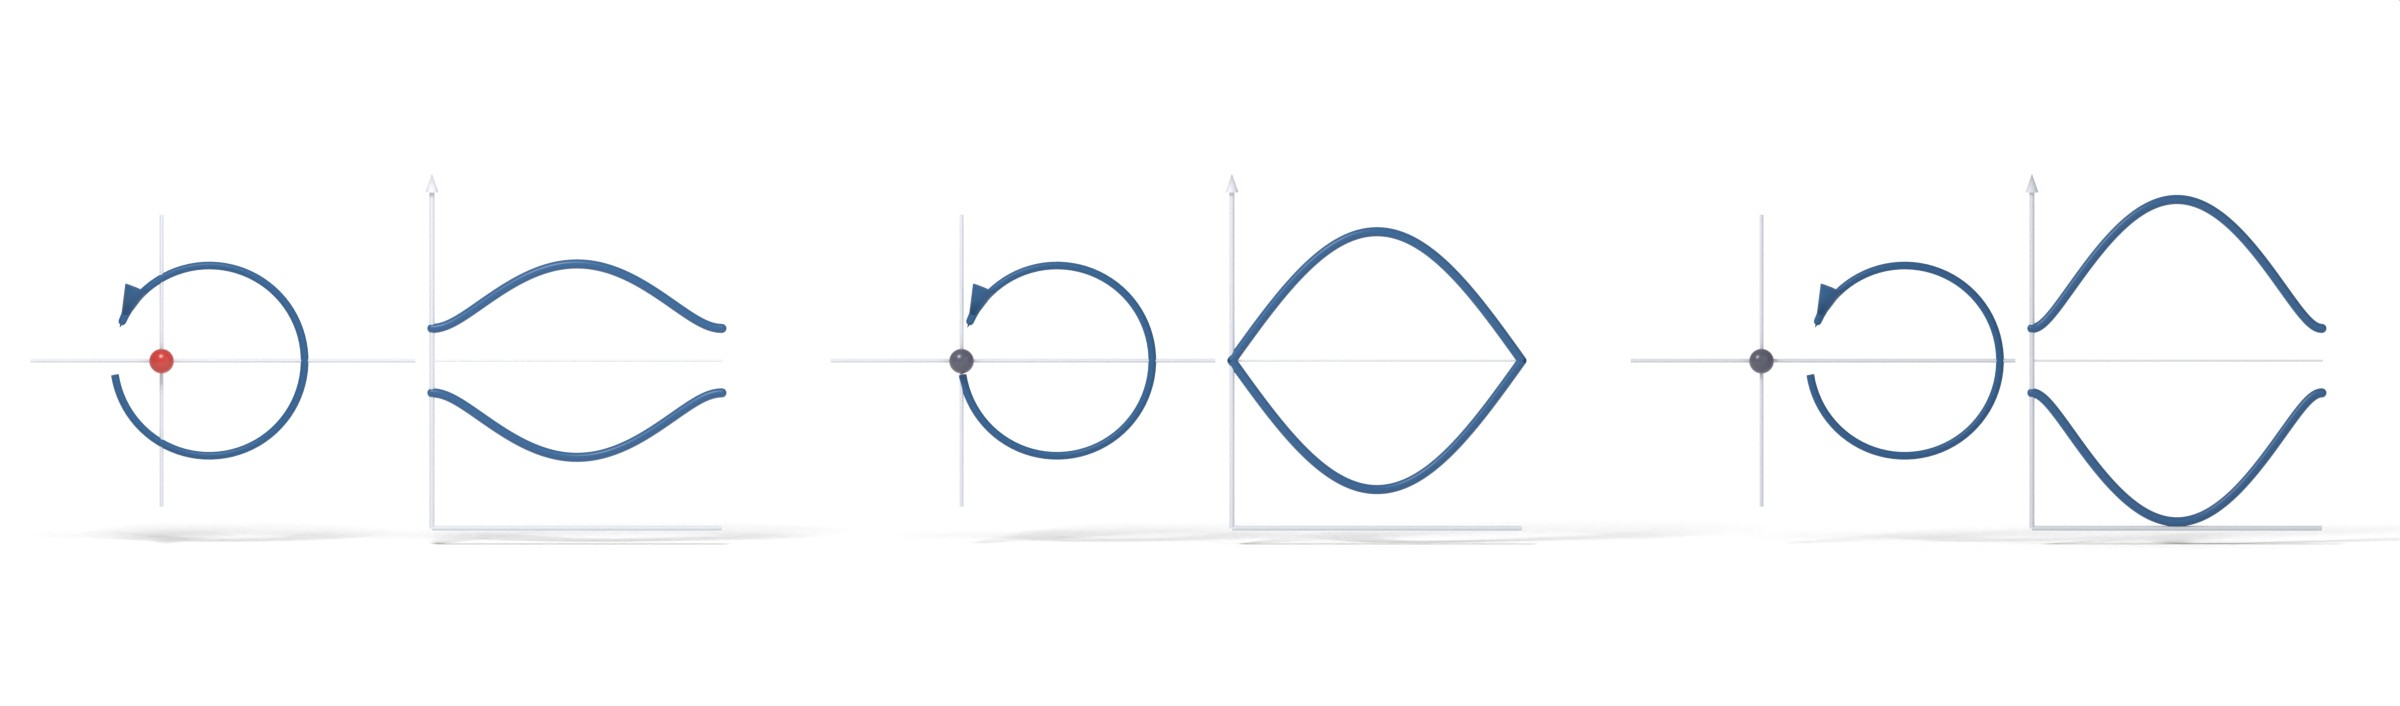
\includegraphics[width=\figw]{../blender/out/s03f04_winding.jpg}};
  % written by build_figure.sh; the painted part of the image
\path (0.0125\figw,0.0667\figw) rectangle (0.9988\figw,0.2217\figw);

  %% written by figlib.py; x and y in units of the image width
\coordinate (azero) at (0.0641\figw,0.1407\figw);
\coordinate (are) at (0.1150\figw,0.1736\figw);
\coordinate (acO) at (0.0673\figw,0.1439\figw);
\coordinate (acre) at (0.1731\figw,0.1439\figw);
\coordinate (acim) at (0.0673\figw,0.2046\figw);
\coordinate (at) at (0.1282\figw,0.2462\figw);
\coordinate (aE) at (0.1800\figw,0.2218\figw);
\coordinate (akmin) at (0.1800\figw,0.0727\figw);
\coordinate (akmax) at (0.3008\figw,0.0727\figw);
\coordinate (agap) at (0.3040\figw,0.1439\figw);
\coordinate (bzero) at (0.3974\figw,0.1407\figw);
\coordinate (bre) at (0.4682\figw,0.1736\figw);
\coordinate (bcO) at (0.4006\figw,0.1439\figw);
\coordinate (bcre) at (0.5064\figw,0.1439\figw);
\coordinate (bcim) at (0.4006\figw,0.2046\figw);
\coordinate (bt) at (0.4615\figw,0.2462\figw);
\coordinate (bE) at (0.5133\figw,0.2218\figw);
\coordinate (bkmin) at (0.5133\figw,0.0727\figw);
\coordinate (bkmax) at (0.6341\figw,0.0727\figw);
\coordinate (bgap) at (0.6373\figw,0.1439\figw);
\coordinate (czero) at (0.7308\figw,0.1407\figw);
\coordinate (cre) at (0.8214\figw,0.1736\figw);
\coordinate (ccO) at (0.7340\figw,0.1439\figw);
\coordinate (ccre) at (0.8397\figw,0.1439\figw);
\coordinate (ccim) at (0.7340\figw,0.2046\figw);
\coordinate (ct) at (0.7949\figw,0.2462\figw);
\coordinate (cE) at (0.8466\figw,0.2218\figw);
\coordinate (ckmin) at (0.8466\figw,0.0727\figw);
\coordinate (ckmax) at (0.9675\figw,0.0727\figw);
\coordinate (cgap) at (0.9707\figw,0.1439\figw);

  \foreach \p/\t/\w in {a/{0.5}/{winding $1$}, b/{1}/{gap closes}, c/{1.5}/{winding $0$}} {
    \node[lbl, anchor=south] at (\p t) {\textbf{(\p)}\quad$t=\t$, \w};
    \node[lbl, anchor=south west, text=aqmaccent] at (\p re) {$d(k)$};
    \node[lbl, anchor=south west] at (\p E) {$E_\pm$};
    \node[lbl, anchor=north] at (\p kmin) {$-\pi$};
    \node[lbl, anchor=north] at (\p kmax) {$\pi$};
  }
  \node[lbl, anchor=north west, yshift=-1pt] at (azero) {$0$};
  \node[lbl, anchor=north east] at (bzero) {$0$};
  \node[lbl, anchor=north east] at (czero) {$0$};
  \node[axlbl, anchor=south east, xshift=1pt, fill=white, fill opacity=0.85, text opacity=1, inner sep=0.8pt] at (acre) {$\mathrm{Re}\,d$};
  \node[axlbl, anchor=west] at (acim) {$\mathrm{Im}\,d$};
  \node[axlbl, anchor=south east, xshift=1pt, fill=white, fill opacity=0.85, text opacity=1, inner sep=0.8pt] at (bcre) {$\mathrm{Re}\,d$};
  \node[axlbl, anchor=west] at (bcim) {$\mathrm{Im}\,d$};
  \node[axlbl, anchor=south east, xshift=1pt, fill=white, fill opacity=0.85, text opacity=1, inner sep=0.8pt] at (ccre) {$\mathrm{Re}\,d$};
  \node[axlbl, anchor=west] at (ccim) {$\mathrm{Im}\,d$};
\end{tikzpicture}
\end{document}
